
%%%%%%%%%%%%%%%%%%%%%%% file typeinst.tex %%%%%%%%%%%%%%%%%%%%%%%%%
%
% This is the LaTeX source for the instructions to authors using
% the LaTeX document class 'llncs.cls' for contributions to
% the Lecture Notes in Computer Sciences series.
% http://www.springer.com/lncs       Springer Heidelberg 2006/05/04
%
% It may be used as a template for your own input - copy it
% to a new file with a new name and use it as the basis
% for your article.
%
% NB: the document class 'llncs' has its own and detailed documentation, see
% ftp://ftp.springer.de/data/pubftp/pub/tex/latex/llncs/latex2e/llncsdoc.pdf
%
%%%%%%%%%%%%%%%%%%%%%%%%%%%%%%%%%%%%%%%%%%%%%%%%%%%%%%%%%%%%%%%%%%%


\documentclass[runningheads,a4paper]{llncs}

\usepackage{amssymb}
\setcounter{tocdepth}{3}
\usepackage{graphicx}

\usepackage{url}
\urldef{\mailsa}\path|{florian.hanika, gerhard.wohlgenannt}@wu.ac.at|
\urldef{\mailsb}\path|marta.sabou@modul.ac.at|
%\urldef{\mailsb}\path|marta.sabou|
%\urldef{\mailsc}\path|{erika.siebert-cole, peter.strasser, lncs}@springer.com|    
\newcommand{\keywords}[1]{\par\addvspace\baselineskip
\noindent\keywordname\enspace\ignorespaces#1}

\begin{document}

\mainmatter % start of an individual contribution

% first the title is needed
%\title{Crowdsourcing Enabled Ontology Engineering}
\title{The uComp Prot\'eg\'e Plugin:\\ Crowdsourcing Enabled Ontology Engineering}
%\title{The uComp Prot\'eg\'e Plugin:\\ Towards Embedded Human Computation for Ontology Engineering}
%Alternatives
%* Crowd-based ontology engineering
%* Tool support for crowd-based ontology engineering
%* The uComp Prot\'eg\'e Plugin: Towards Embedded Human Computation for Ontology Engineering
%* Enabling Embedded Human Computation in Ontology Engineering with the uComp Prot\'eg\'e Plugin

% a short form should be given in case it is too long for the running head
\titlerunning{Crowdsourcing Enabled Ontology Engineering}

% the name(s) of the author(s) follow(s) next
%
% NB: Chinese authors should write their first names(s) in front of
% their surnames. This ensures that the names appear correctly in
% the running heads and the author index.
%
\author{Florian Hanika\inst{1}
\and Gerhard Wohlgenannt\inst{1}
\and Marta Sabou\inst{2}}

%
\authorrunning{Hanika et al.}
% (feature abused for this document to repeat the title also on left hand pages)

% the affiliations are given next; don't give your e-mail address
% unless you accept that it will be published

\institute{WU\
Vienna\\
\mailsa\\
%\url{http://www.wu.ac.at}
\and
MODUL University Vienna\\
\mailsb\\
%\url{http://modul.ac.at}
}




%\author{Ivar Ekeland\inst{1} \and Roger Temam\inst{2}
%Jeffrey Dean \and David Grove \and Craig Chambers \and Kim~B.~Bruce \and
%Elsa Bertino}
%
%\institute{Princeton University, Princeton NJ 08544, USA,\\
%\email{I.Ekeland@princeton.edu},\\ WWW home page:
%\texttt{http://users/\homedir iekeland/web/welcome.html}
%\and
%Universit\'{e} de Paris-Sud,
%Laboratoire d'Analyse Num\'{e}rique, B\^{a}timent 425,\\
%F-91405 Orsay Cedex, France}

%
% NB: a more complex sample for affiliations and the mapping to the
% corresponding authors can be found in the file "llncs.dem"
% (search for the string "\mainmatter" where a contribution starts).
% "llncs.dem" accompanies the document class "llncs.cls".
%

%\toctitle{Lecture Notes in Computer Science}
%\tocauthor{Authors' Instructions}
\maketitle


\begin{abstract}

%Embedded Human Computation advocates a tight integration of Human Computation (HC) methods into computational workflows. 
%HC used a lot in OE with good results, but now time to move.
%In this paper we discuss two enabling elements for EHC in the domain of ontology engineering. Firstly, we show that a set of basic HC tasks are used recurrently to solve a range of ontology engineering tasks. Secondly, we present the \textit{uComp Prot\'eg\'e plugin} that facilitates the integration of such typical HC tasks into the ontology engineering process from within the ontology editing environment in the spirit of EHC. An evaluation of the plugin in a typical ontology engineering scenario where ontologies are built from automatically learned semantic structures, shows that its use reduces the working times for the ontology engineers 11 times, reduces the overall task costs with 40\% to 83\% depending on the HC settings used and leads to data quality comparable with that of tasks performed by ontology engineers. 

% is an emerging trend that moves beyond the use of HC methods for data acquisition towards their


%Since HC methods have been already successfully used to solve various OE tasks, their tighter integration into OE processes high adoption and routine inclusion 

%The successful use of Human Computation (HC) to solve various ontology engineering tasks (e.g., vocabulary building, ontology alignment) 

%makes it logical to tightly couple such methods into ontology engineering workflows, a novel paradigm we call Embedded Human Computation (EHC). 
%
%Which HC tasks are most frequently used? How to support ontology experts without much HC knowledge to solve parts of their ontology engineering tasks using HC?

%The development of this novel paradigm, is however currently hampered by 1) a lack of understanding of which HC tasks are most often used in the ontology engineering process and 2) tool support in ontology engineering platforms that would allow easy insertion of HC into ontology engineering workflows.

%TBD: clarify novelty (e.g., which new tasks we introduce?), sum up some important evaluation results.

Crowdsourcing techniques have been shown to provide effective means for solving a variety of ontology engineering problems. Yet, they are mainly being used as external means to ontology engineering, without being closely integrated into the work of ontology engineers. In this paper we investigate how to closely integrate crowdsourcing into ontology engineering practices.
Firstly, we show that a set of basic crowdsourcing tasks are used recurrently to solve a range of ontology engineering problems. Secondly, we present the \textit{uComp Prot\'eg\'e plugin} that facilitates the integration of such typical crowdsourcing tasks into ontology engineering work from within the Prot\'eg\'e ontology editing environment. An evaluation of the plugin in a typical ontology engineering scenario where ontologies are built from automatically learned semantic structures, shows that its use reduces the working times for the ontology engineers 11 times, lowers the overall task costs with 40\% to 83\% depending on the crowdsourcing settings used and leads to data quality comparable with that of tasks performed by ontology engineers. 

%use by ontology engineers is not straightforward.
\keywords{crowdsourcing, ontology engineering, ontology learning, Prot\'eg\'e plugin}
\end{abstract}


\section{Introduction}

%Context & Scenario
Ontology engineering consists of a collection of knowledge acquisition and management techniques for creating and maintaining ontologies during their entire life-cycle. %thus being a crucial component of any Semantic Web based system. 
Ontology engineering tasks tend to be complex, costly and, above all, time-consuming processes.

Let's consider the task of ontology creation. To reduce its complexity, ontology construction is often bootstrapped by re-using existing or automatically derived ontologies. % derived by automatic methods from non-ontological resources (e.g., text corpora, folksonomies). 
Ontology learning methods, for example, automatically extract ontologies from (a combination of) unstructured and structured resources. Although the extracted ontologies already provide a good basis for building the ontology, they typically contain questionable or wrong ontological elements and require a phase of verification and redesign (especially pruning) by the ontology engineer. The ontology verification phase involves, among others, checking that the ontology concepts are relevant to the domain of interest and that the extracted subsumption relations are correct. %Since the uComp plugin supports these tasks, we will evaluate them in an ontology engineering scenario by reusing automatically learned ontologies. % obtained through ontology learning.

%CS can be used for KA
%Crowdsourcing methods have been used to solve a range of knowledge acquisition tasks, in general~\cite{Sabou2013} and ontology engineering tasks in particular as discussed in Section~\ref{ss:HCKAq}. 
Crowdsourcing methods provide effective means to solve such ontology verification tasks by outsourcing these to ``an undefined, generally large group of people in the form of an open call"~\cite{Howe2009}. As detailed in Section~\ref{ss:HCKAq}, crowdsourcing has been used effectively to solve a range of ontology engineering tasks. However, crowdsourcing techniques require high upfront investments (understanding the techniques, creating appropriate tasks) and therefore, despite their proven usefulness, these techniques remain outside the reach of most ontology engineers. 
%Attempts to address this situation include, for example, WebProt\'eg\'e~\cite{Tudorache2013} - an extension of the Prot\'eg\'e ontology editor that opens up the ontology engineering process to a larger, distributed group of contributors. Similarly, in the area of natural language processing, GATE Teamware extends the GATE linguistic annotation toolkit with distributed knowledge creation capabilities~\cite{Bontcheva2013}.While these extensions primarily support the collaborative and distributed work of knowledge experts (ontology engineers and linguists), an increasing trend is allowing large populations of \textit{non-experts} to create knowledge through the use of Human Computation platforms such as games or mechanised labour platforms.
%Some of the newer approaches, such as ZenCrowd~\cite{Demartini2012} and CrowdMap~\cite{Sarasua2012}, are making a move towards a tighter integration of HC methods into computational workflows to solve Semantic Web specific tasks such as entity linking or ontology matching. 

In this paper we investigate how to more closely embed crowdsourcing into ontology engineering. In the area of Natural Language Processing (NLP), where the use of crowdsourcing is highly popular~\cite{Sabou_Bontcheva_Scharl_2012}, there already exists an effort towards supporting easy integration of crowdsourcing methods into linguists' work: the GATE Crowdsourcing Plugin is a new component in the popular GATE NLP platform that allows inserting crowdsourcing tasks into larger NLP workflows, from within GATE's user interface~\cite{Bontcheva2014}. %After concluding that micro-workers are a viable alternative for verifying subclass-superclass relations, 
Noy and colleagues~\cite{Noy2013} introduce a vision for similar tool support to facilitate the integration of crowdsourcing into ontology engineering. To achieve our goal we seek answer to two research questions:

\begin{description}
\item [Which tasks can be crowdsourced?] We distill a set of crowdsourcing tasks that are likely to be common to solving a variety of ontology engineering problems and which should be implemented by the desired tool support (Section~\ref{ss:HCKAq}).

\item [How to implement crowdsourcing enabled ontology engineering?] We\\ present a tool, the uComp Prot\'eg\'e plugin, which allows ontology engineers to crowdsource tasks directly from within the popular ontology engineering tool and as part of their ontology engineering work (Section~\ref{s:plugin}).
\end{description}
%\end{enumerate}

We evaluate some of the functionality of the plugin to estimate the improvements made possible over manually solving a set of tasks in terms of time and cost reductions, while maintaining good data quality (Section~\ref{sec:eval}). Our findings show that, in a scenario where automatically extracted ontologies are verified and pruned, the use of the plugin significantly reduces the time spent by the ontology engineer (11 times) and leads to important cost reductions (40\% to 83\% depending on the crowdsourcing settings used) without a loss of quality with respect to a manual process.

\section{Use of Crowdsourcing for Knowledge Acquisition}\label{ss:HCKAq}

Crowdsourcing methods are usually classified in three major genres depending on the motivation of the human contributors (i.e., payment vs. fun vs. altruism). 
%Human Computation (HC) describes systems that combine automated methods with large numbers of human contributors who collaborate to perform a task, typically involving an automated system that serves up task instances and then aggregates the produced results~\cite{Quinn2011}. HC systems are classified in three major genres depending on the motivation of the human contributors (e.g., payment vs. fun vs. altruism).
% HC tasks usually have an artificial intelligence flavour, with the humans being needed to perform a sub-task for which effective algorithms are not yet available. HC includes a number of genres, which can be distinguished along various dimensions, such as the motivation of human contributors (e.g., entertainment, altruism, payment) and skills required, how individual results are aggregated and how quality is managed [35]. Key HC genres include crowdsourcing, mechanised labour (e.g. Amazon Mechanical Turk), and games with a purpose (GWAP), where human contributors are motivated by formulating tasks as enjoyable games [21]. 
 Mechanised labour (MLab) is a type of paid-for crowdsourcing, where contributors choose to carry out small tasks (or micro-tasks) and are paid a small amount of money in return.
 % The most popular platform for mechanised labour is Amazon's Mechanical Turk (MTurk) which allows requesters to post their micro-tasks in the form of Human Intelligence Tasks (or HITs) to a large population of micro-workers (often referred to as �turkers�). 
Popular crowdsourcing marketplaces include Amazon's Mechanical Turk (MTurk) and CrowdFlower (CF). Games with a purpose (GWAPs) enable human contributors to carry out computation tasks as a side effect of playing online games~\cite{vonAhn2008}. % An example from the area of computational biology is the Phylo game (phylo.cs.mcgill.ca) that disguises the problem of multiple sequence alignment as a puzzle like game thus �intentionally decoupling the scientific problem from the game itself� (Kawrykow et al, 2008). The challenges in using GWAPs in scientific context are in designing appealing games and attracting a critical mass of players.
Finally, in altruistic crowdsourcing a task is carried out by a large number of volunteer contributors. %, such as in the case of the Galaxy Zoo (www.galaxyzoo.org) project where over 250K volunteers willing to help with scientific research classified Hubble Space Telescope galaxy images (150M galaxy classifications). 
Crowdsourcing methods have been used to support several knowledge acquisition and, more specifically, ontology engineering tasks. To provide an overview of these methods we will group them along the three major stages of the Semantic Life-cycle as identified by Siorpaes in~\cite{Siorpaes2008} %, where Stage 1 and 2 cover our notion of ontology engineering [TBD - clarify]. 
and sum them up in Table \ref{table:tasksFromRW}.\\

\noindent \textbf{Stage 1: Build and maintain Semantic Web vocabularies}  Eckert and colleagues~\cite{Eckert2010} relied on MTurk micro-workers to build a concept hierarchy in the philosophy domain. Crowdsourcing complemented the output of an automatic hierarchy learning method in: a) judging the relatedness of concept pairs %(on a 5-points scale between unrelated and related)
 and b) specifying the level of generality between two terms (more/less specific than). 
Noy and colleagues~\cite{Noy2013} focused on verifying the correctness of taxonomic relations. %subclass-superclass relations that make up the ontology hierarchy as a critical task while building ontologies. 
%Eckert - end goal: construction of hierarchies by aggregating human expert feedback on the relatedness and relative generality of terms; domain philosophy; Similar to us: "automatic OL methods are often weak on the task of determining the type of relation that holds between two terms" - I do not understand all details here ...
%GWAPs have also been used in ontology creation. 
%OntoPronto - decide whether a term is a class or an instance; then they relate this class to the most specific relevant PROTON class, therefore extending PROTON
As for GWAPs, the OntoPronto game~\cite{Siorpaes2008} aims to support the creation and extension of Semantic Web vocabularies. Players are presented with a Wikipedia page of an entity and they have to (1) judge whether this entity denotes a concept or an instance; and then (2) relate it to the most specific concept of the PROTON ontology, therefore extending PROTON with new classes and instances. Climate Quiz~\cite{Scharl2012a} is a Facebook game where players evaluate whether two concepts are related (e.g. �environmental activism�, �activism�), and which label is the most appropriate to describe their relation. The possible relation set contains both generic (�is a sub-category of�, �is identical to�, �is the opposite of�) and domain-specific (�opposes�, �supports�, �threatens�, �influences�, �works on/with�) relations. %Two further relations, �other� and �is not related to� were added for cases not covered by the previous eight relations. The game�s interface allows players to switch the position of the two concepts or to skip ambiguous pairs.
Guess What?!~\cite{Markotschi2010} goes beyond eliciting or verifying relations between concepts to creating complex concept definitions. %The game explores instance data available as linked open data. Given a seed concept (e.g., banana), the game engine collects relevant instances from DBpedia, Freebase and OpenCyc and extracts the main features of the concept (e.g., fruit, yellowish) which are then verified through the collective process of game playing. The tasks performed by players are: 
Players (1) assign a class name to a complex class description (e.g., assign $Banana$ to $fruit \& yellow \& grows\ on\ trees$) and (2) verify such class definitions.\\

\noindent \textbf{Stage 2: Align Semantic Web vocabularies}
The CrowdMap system enlists micro-workers to solve the ontology alignment task~\cite{Sarasua2012} by asking them to 1) verify whether a given relation is correct (e.g., ``Is conceptA the same as conceptB? yes/no ") and 2) specify how two given terms are related, in particular by choosing between sameAs, isAKindOf and notRelated. %CrowdMap is designed to allow sameAs, subsumption or generic mappings between classes, properties and axioms, but currently it only supports equivalence and subsumption mappings between classes. 
SpotTheLink has been instantiated to align the eCl@ss and UNSWPC~\cite{Siorpaes2008} as well as the DBpedia and PROTON ontologies~\cite{Thaler2011a}. The final version of the game solves ontology alignment through two atomic tasks: (1) choosing a related concept -- given a DBpedia concept players choose and agree upon a related PROTON concept; (2) specifying the type of relation between two concepts.% in terms of equivalence or subsumption.\\
\\
%[TBD if time and place] Community focused efforts in Noy2013

\noindent \textbf{Stage 3: Annotate content and maintain annotations} In ZenCrowd~\cite{Demartini2012} crowd-workers verify the output of automatic entity linking algorithms. Concretely, given a named entity, e.g., ``Berlin", and a set of DBpedia URLs generated automatically, crowd-workers choose all the URLs that represent that entity or ``None of the above" if no URL is suitable. In essence, this is an annotation task. WhoKnows?~\cite{Waitelonis2011} and RISQ!~\cite{Wolf2011} are GWAPs which rely on similar mechanisms: they use LOD facts to generate questions and use the answers to (1) evaluate property rankings (which property of an instance is the most important/relevant); (2) detect inconsistencies; and (3) find doubtful facts. %The obtained property rankings reflect the �wisdom of the crowd� and are an alternative to semantic rankings generated algorithmically based on statistical and linguistic techniques. The games differ in the gaming paradigm they adopt. 
While WhoKnows?! uses a classroom paradigm and aims towards being an educational game, RISQ! is a Jeopardy-style quiz game. 

%[TBD: More: Celino; Sioarpaes ebay and video annotations]

\begin{table}
%\footnotesize

\center
\begin{tabular}{|l|l|c|c|} \hline
\textbf{SW Life-cycle}&\textbf{Approach}&\textbf{Genre}& \textbf{Solved Task}\\ 
\textbf{Stage}&&&\\ \hline


Stage 1: Build and & InPho~\cite{Eckert2010} & MLab & (T3) Specification of Relation Type (subs)\\ 
\cline{4-4}
	maintain 				 & & & (T1) Specification of Term Relatedness \\ 
					 
 \cline{2-4}
					 
Semantic Web & Noy~\cite{Noy2013} & MLab & (T2) Verification of Relation Correctness (subs) \\ 

 \cline{2-4}
vocabularies & OntoPronto~\cite{Siorpaes2008} & GWAP & Class vs. instance decisions \\ 
 \cline{4-4}
 &&& (T3) Specification of Relation Type (subs/instOf) \\ 
 \cline{2-4}
 
&Climate Quiz~\cite{Scharl2012a} & GWAP & (T3) Specification of Relation Type (8 relations) \\
 \cline{2-4}
 
&Guess What?!~\cite{Markotschi2010}& GWAP & Verify complex class definitions \\ 
 \cline{2-4}
& & & Generate class names for complex defs \\ \hline
 Stage 2: Align &CrowdMap~\cite{Sarasua2012} & MLab & (T2) Verification of Relation Correctness (subs/eqv) \\
 \cline{4-4}
Semantic Web & && (T3) Specification of Relation Type (subs/eqv) \\ 
 \cline{2-4}
vocabularies &SpotTheLink~\cite{Thaler2011a} & GWAP & (T1) Specification of Term Relatedness \\
 \cline{4-4}
& & & (T3) Specification of Relation Type (subs/eqv) \\ 
 \hline
Stage 3: Annotate & ZenCrowd~\cite{Demartini2012} & MLab & Text to URL mapping (annotation) \\
 \cline{2-4}
content, maintain & WhoKnows?~\cite{Waitelonis2011}& GWAP& Answering quiz questions\\
 \cline{2-4}
annotations &RISQ!~\cite{Wolf2011}&GWAP& Answering quiz questions\\ \hline

\end{tabular}
\caption{Overview of approaches addressing problems in various stages of the Semantic Web life-cycle~\cite{Siorpaes2008}, their genres and the type of crowdsourcing tasks that they employ.}
\center \label{table:tasksFromRW}
\end{table}


 \subsection{Typical Crowdsourcing Tasks in Ontology Engineering}\label{ss:crowdtasks}

Based on the analysis above, we distill a set of recurrent basic crowdsourcing task types used to solve a variety of ontology engineering problems, as follows.\\ %of the crowdsourcing methods used to support ontology engineering tasks, it emerges that they often converge towards using a range of typical crowdsourcing tasks as follows. 

\begin{description}
\item[T1. Specification of Term Relatedness.] Crowd-workers judge whether two terms (typically representing ontology concepts) are related. In some cases they are presented with pairs of terms~\cite{Eckert2010} while in others they might need to choose a most related term from a set of given terms~\cite{Thaler2011a}. This type of crowdsourcing task is suitable both in ontology creation~\cite{Eckert2010} and in ontology alignment scenarios~\cite{Thaler2011a}. 

\item[T2. Verification of Relation Correctness.] Presented with a pair of terms (typically representing ontology concepts) and a relation between these terms, crowd-workers judge whether the suggested relation holds. Frequently verified relations include generic ontology relations such as equivalence~\cite{Sarasua2012} and subsumption~\cite{Noy2013,Sarasua2012}, which are relevant both in ontology evaluation~\cite{Noy2013} and ontology alignment scenarios~\cite{Sarasua2012}. 

\item[T3. Specification of Relation Type.] In these tasks, crowd-workers are presented with two terms (typically corresponding to ontology concepts) and choose an appropriate relation from a set of given relations. Most efforts focus on the specification of generic ontology relations such as equivalence ~\cite{Scharl2012a,Sarasua2012,Thaler2011a}, subsumption~\cite{Scharl2012a,Eckert2010,Siorpaes2008,Sarasua2012,Thaler2011a}, disjointness~\cite{Scharl2012a} or instanceOf~\cite{Siorpaes2008,Scharl2012a}. The verification of domain-specific named relations such as performed by Climate Quiz~\cite{Scharl2012a} is less frequent. 

% [BTW, since this is a complex task it could be split up into a sequence of 3 simpler tasks: 1) given two terms workers agree whether these are related or not; 2) those pairs that were judged related are then passed to another task where a correct relation is selected; 3) in the third task, the quality of the relations is checked - practically T2] Available relation labels are some predefined (like subClassOf) and those from the target ontology (all ObjectProperties) -- if more than 20 .. spread over multiple windows (depending on window size) Have a limit of 5 relation labels in the Prot\'eg\'e interface All pairs with a certain relation (defined by the user in a text field, eg �relation�) are sent to the uComp API (or directly to CF). If you want to use just a subset of relations: have a window where you select (checkboxes) the actual pair to be sent. In CrowdFlower -- also have the choice to add a free text label output: be able to sort by certainty from CF ..

 %This is also a very difficult task in OL in general - the
\item[T4. Verification of Domain Relevance.]  For this task, the crowdworkers confirm whether a given term is relevant for a domain of discourse. This task is mostly needed to support scenarios where ontologies are extracted using automatic methods, for example, through ontology learning. \\
\end{description} 


The core crowdsourcing tasks above have been used by several approaches and across diverse stages of ontology engineering, thus being of interest in a wide range of ontology engineering scenarios. As such, they guided the development of our plugin, which currently supports tasks T2, T4, and partially T3.


\section{The uComp Prot\'eg\'e Plugin}~\label{s:plugin}

In order to support ontology engineers to easily and flexibly integrate crowdsourcing tasks within their work, we implemented a plugin in Prot\'eg\'e, one of the most widely used ontology editors. The typical workflow of using the plugin involves the following main stages (as also depicted in Figure~\ref{fig:process}).

\begin{figure*}[htb]
\centering
{\centering \resizebox*{1.0\textwidth}{!}{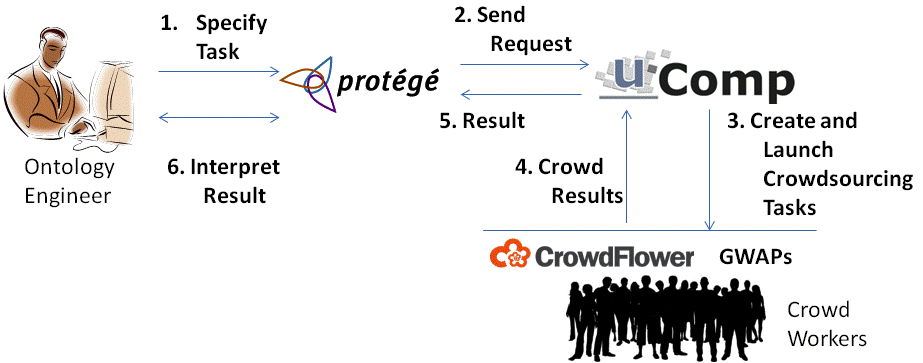
\includegraphics{images/process.png}}}
 \caption{\label{fig:process} Main stages when using the uComp plugin.}
\end{figure*}


\begin{description}
\item[1. Task Specification.] An ontology engineer using Prot\'eg\'e can invoke the functionalities of the plugin from within the ontology editor at any time within his current work. The plugin allows specifying some well defined ontology engineering tasks, such as those discussed in Section~\ref{ss:crowdtasks} above. The view of the plugin that is appropriate for the task at hand is added to the editor's user interface via the \emph{Window $\rightarrow{}$ Views} menu. The ontology engineer then specifies the part of the ontology to verify (eg. a specific class or all classes in the ontology), provides additional information and options in the plugin view and then starts the evaluation. Crowdsourced tasks can be canceled (or paused) anytime during the crowdsourcing process. We further detail the plugin's functionality in Section~\ref{ss:functionality}.

\item[2. Task Request.] The plugin uses the uComp API\footnote{\url{http://tinyurl.com/uCompAPI}} to request the processing of the task by the crowd.

\item[3. Creation of Crowdsourcing Tasks.] The crowdsourcing process happens through the uComp platform\footnote{The platform is being developed in the uComp project (\url{http://www.ucomp.eu/})}, a hybrid-genre crowdsourcing platform which facilitates various knowledge acquisition tasks by flexibly allocating the received tasks to GWAPs and/or mechanised labour platforms alike (in particular, CrowdFlower)~\cite{Sabou2013} depending on user settings.%, the uComp platform delegates the job to a GWAP, to CrowdFlower or to a combination of these two genres. In Section~\ref{ss:crowdtasks} we present the crowdsourcing tasks created by the uComp platform.

%NEW_wohlg -- extended (R1 last paragraph) version
\item[4. Collection of Crowd Results.] The uComp platform collects crowd-work harvested by individual genres (GWAPs and micro-task crowdsourcing).


\item[5. Combination of Crowd Results.] 
When all crowdsourcing tasks of a job have completed, the platform combines the results and provides them to the plugin.


% orig version (before 2014-09-17)
% \item[4\&5 Collection of Crowd Results.] The uComp platform collects crowd-work harvested by various genres in step 4.
%When all task have completed, the platform combines the results and provides them to the plugin (step 5). 



\item[6. Result Presentation and Interpretation.] As soon as available, the plugin presents the results to the ontology engineer and saves them in the ontology. All data collected by the plugin %which should be persistent [TBD - what is persistent?]
is stored in the ontology in \texttt{rdfs:comment} fields, for example information about the ontology domain, the crowdsourcing job ID, and the crowd-created results. Depending on the result, the ontology engineer will perform further actions such as deleting parts of the ontology which have been validated as non-relevant.
\end{description}

\subsection{Plugin Functionality}\label{ss:functionality}

The plugin provides a set of views for crowdsourcing the following tasks:

%COMMENT: maybe we should switch to a more OWL/Protege-ish terminology (as suggested by R2). Relation -> property, ... (see his "minor comments")
\begin{itemize}
\item Verification of Domain Relevance (T4)
\item Verification of Relation Correctness - Subsumption (T2)

\item Verification of Relation Correctness - InstanceOf (T2) - the verification of \emph{instanceOf} relations between an individual and a class.%, i.e.~the crowd helps to verify if a given \emph{instanceOf} is valid.

\item Specification of Relation Type (T3) is a Prot\'eg\'e view component that collects suggestions for labeling unlabeled relations by assigning to them a relation type from a set of relation types specified by the ontology engineer.

%COMMENT: changed "restrictions" to "axioms" (R2)
\item Verification of Domain and Range where crowd-workers validate whether a property's \emph{domain} and \emph{range} axioms are correct.
%This results in two separate sub-tasks (domain, range). [<=TBD: what does this do exactly] 

\end{itemize}


In this paper we focus on the first two functionalities, which we now describe in more detail.

%Florian: The CF key has to be associated with the uComp-API key, therefore it has to be communicated to the uComp-API team (see http://soc.ecoresearch.net/facebook/election2008/ucomp-quiz-beta/api/v1/documentation/)
%Florian: The uComp-API key itself must be put into a textfile named "ucomp_api_key.txt" at the users home directory, in the folder ".Protege" (which is created by Prot\'eg\'e during installation on both Windows and Linux plattforms) 

%Florian: all information about the task is stored (depends on the kind of task): domain, validation of whole subtree going on?, additional information, sent to crowdflower or ucomp-quiz, ucomp-api job-id, ...

% give an example SCREEENSHOT with a quick introduction 
\begin{figure*}[htb]
\centering
{\centering \resizebox*{1.0\textwidth}{!}{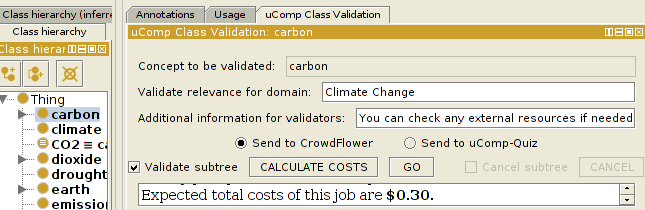
\includegraphics{images/cc_class.png}}}
 \caption{\label{fig:screen_cr} The interface of the uComp Class Validation view used to create a Verification of Domain Relevance (T4) task.} %TBD: Gerhard: could you make a new screenshot, with another term that is more know and also shown highlighte in the left side hierarchy list - "climate" would be great. Also, can you add some example text in "Additional information for validators": for example: "You can check any external resources if needed."}
\end{figure*}
%[TBD: Gerhard: could you make a new screenshot, with another term that is more know and also shown highlighte in the left side hierarchy list - "climate" would be great. Also, can you add some example text in "Additional information for validators": for example: "You can check any external resources if needed."]



% COMMON FIELDS in the UI: domain and additional information & validate subtree
% TASKs
\textbf{Verification of Domain Relevance (T4)} is supported by the ``uComp Class Validation'' view of the plugin and crowdsources the decision of whether a concept (class) is relevant for a domain. %First, the ontology engineer adds the corresponding view (\emph{Window} $\rightarrow{}$ \emph{Views} $\rightarrow{}$ \emph{Class Views} $\rightarrow{}$ \emph{uComp Class Validation}) to the editor's UI. 
Figure~\ref{fig:screen_cr} shows the screenshot of this view for the class ``carbon'' before initiating the verification. 
%[TBD - how does the returned result look like? Do we have a screenshot?] 
The plugin view's interface contains the following information:

\begin{description}
\item[Task Specific Information] such as the concept selected by the user for validation. This part of the view is diverse among different plugin functionalities.
\item[Generic information] such as the \emph{domain} of the ontology, i.e., the field of knowledge which the ontology covers, is present in all views of the plugin. If entered once, the domain will be stored in the ontology (as \texttt{rdfs:comment}) and be pre-filled subsequently, but it can also be changed at any time.
\item[Additional information] For every task, the plugin contains a predefined task description (typically including examples) which is presented to the crowd-worker. If the ontology engineer wants to extend this task description, (s)he can provide more guidelines in the \emph{additional information} field. This functionality is present in all the views of the plugin.
\item[Recursive control] allows performing a task (e.g., domain relevance validation) not only for the current class, but for a larger part of or even the entire ontology. If the \emph{Validate subtree} option is selected, the plugin crowdsources the specified task for the current concept and all its subconcepts recursively. To apply the functionality to the entire ontology, the plugin is invoked from the uppermost class, i.e., (\emph{Thing}).
\item[\texttt{GO} button] to start the crowdsourcing process. 
\end{description}


%Florian: domain will be stored as rdfs:comment in the head of the ontology

% T1. Verification of Domain Relevance. Is a concept/instance relevant for a domain?
% T2. Verification of Relation Correctness. Does a certain relation between two ontology entities hold? These could be a set of generic relations (sameAs, subClassOf, instanceOf), but also arbitrary named relations to be specified by the ontology engineer. The crowd here would have to vote (yes/no) for a given triple (Subject - Relation - Object). This task is the focus of [1].

\begin{figure*}[htb]
\centering
{\centering \resizebox*{1.00\textwidth}{!}{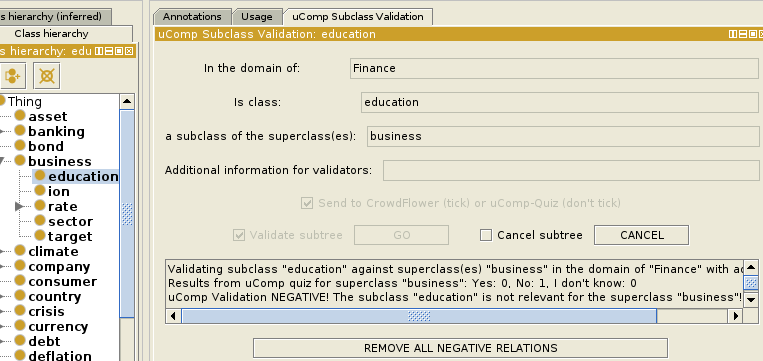
\includegraphics{images/sc_subclass_val.png}}}
 \caption{\label{fig:screen_sub}Screenshot showing the interface for subClassOf relation validation, including the display of results.}
\end{figure*}


\textbf{Verification of Relation Correctness - Subsumption (T2).}
%The second task is the verification of relation correctness, more precisely the verification of IS-A (subClassOf) relations between classes. The corresponding view is named 
 is achieved with the \emph{uComp SubClass Validation}. When selecting a class in Prot\'eg\'e,
the plugin automatically detects its superclasses (if any) and fills the boxes in the plugin UI.
%NEW_wohlg (next sentence):
As with any plugin functionality, the elements of the user interface are described in the plugin documentation, and additional information is also given interactively as mouse-over overlays.
%Additional information about the elements of the interface are presented to the user as mouse-over 
As soon as results are available these are presented in the UI, as shown in Figure~\ref{fig:screen_sub}. The screenshot gives an example
with one evaluator, who rated the \emph{IS-A} relation between ``education'' and ``business'' as invalid. If the majority of judgements is negative,
a button to remove the relation is displayed.

\subsection{Crowdsourcing Task Interfaces}\label{ss:crowdtasks}

Upon receiving the request from the Prot\'eg\'e plugin, the uComp API selects the appropriate crowdsourcing genre and creates the relevant crowd-jobs. Currently the platform can crowdsource tasks either to GWAPs such as Climate Quiz~\cite{Scharl2012a} or to CrowdFlower, with a hybrid-genre strategy currently being developed. In this paper, we test the plugin by crowdsourcing only through CrowdFlower. 

Figure~\ref{fig:CFUI} depicts the crowdsourcing interfaces created automatically by the uComp platform for the two tasks discussed above, namely the verification of domain relevance (part a) and the validation of subsumption relations (part b) . 
%COMMENT: not sure if the next sentence is correct -- ie if the uComp API or the Protege plugin will provide the gold units => %MS let's leave this here as it is a small thing
The uComp platform requires only the task data from the Prot\'eg\'e plugin and it provides relevant instructions as well as gold units to all tasks. 
Additionally, each crowdsourcing interface is extended with straightforward verification questions (i.e., typing some letters of the input terms). It has been shown experimentally (e.g.~\cite{Kittur2008,Laws2011}), that extending task interfaces with explicitly verifiable questions forces workers to process the content of the task and also signals to them that their answers are being scrutinized. %This seemingly simple technique had a significant positive effect on the quality of the collected data~\cite{Kittur2008,Laws2011}.

\begin{figure}%[htbp]
 \centering
  \begin{tabular}{c c}
  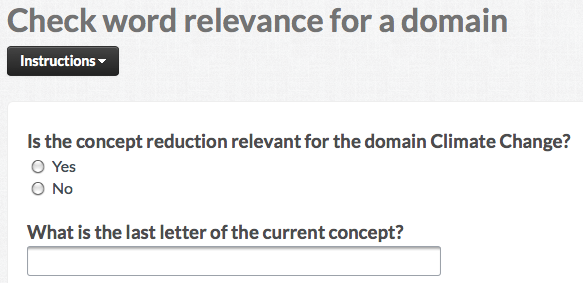
\includegraphics[scale=0.27]{images/CFdomainRel.png}&
  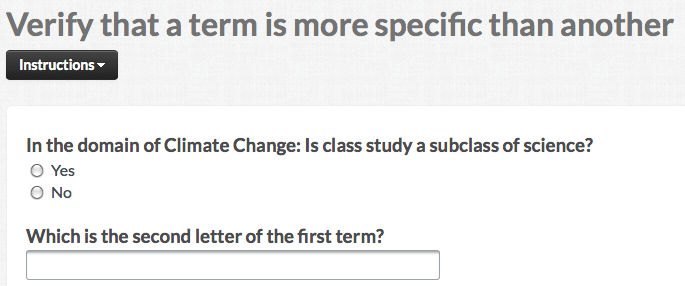
\includegraphics[scale=0.27]{images/CFsubclasscheck.png}\\
  (a) & (b)
  \end{tabular}
  \caption{Generated CrowdFlower job interface for (a) the Verification of Domain Relevance (T4) and (b) the Verification of Relation Correctness (T2) tasks.}
  \label{fig:CFUI}
\end{figure}


To ensure a good quality output, by default all created jobs are assigned to Level 3 CrowdFlower contributors which are the contributors delivering, on average, the highest quality work. Also, for the moment we assume that the verified ontologies will be in English and therefore we restrict contributors to the main English speaking countries: Australia, United Kingdom and United States. In each created job we present 5 units per page and for each unit we collect 5 individual judgements. A price per task of \$0.05 was specified for all jobs.
A task is complete when all requested judgments have been collected.


% Future versions of the plugin will provide higher control over task settings from within Prot\'eg\'e.


%\subsection{Implementation and Installation Details} 
% Prot\'eg\'e can easily be extended in the form of \emph{plugins} which are typically Java Archive (.jar) files
%stored in the Prot\'eg\'e \texttt{plugin} directory. The most common form of a Prot\'eg\'e plugin is a \emph{view plugin}, which implements a single view for a specific area of an ontology (e.g. classes, individuals, object properties).
%Florian: Prot\'eg\'e completely was programmed in Java, therefore all plugins also are programmed in Java. Since Prot\'eg\'e was developed very modular, it is quite easy to create simply plugins and integrate them into Prot\'eg\'e. 
%Florian: All Prot\'eg\'e plugins are so called jar-Files (Java Archive), and contains the compiled source code and all needed libraries. The most common form of a Prot\'eg\'e plugin is a view plugin, which implements a single view for a specific area of an ontology (e.g. classes, individuals, object properties, ...)

% installation / SETUP 
%\textbf{Installation and setup.}
The plugin is available from Prot\'eg\'e's central registry % and can be installed from within Prot\'eg\'e with the \emph{File $\rightarrow{}$ Check for Updates} menu item. A window entitled \emph{Automatic Update} will pop up, where
as the \emph{uComp Crowdsourcing Validation plugin}. % can be selected from the list of downloads. The download files contain the plugin itself, and a detailed documentation.
% NEW_wohlg (next sentence):
The plugin has been tested with Prot\'eg\'e versions 4.2 and 4.3, as well as the recent version 5.0 (beta).
A local configuration file contains the uComp-API key\footnote{Request a key from the uComp team, see \url{http://tinyurl.com/uCompAPI}} and various adaptable settings (e.g., judgements per unit, price per unit).

%To use the plugin a uComp-API key\footnote{Request a key from the uComp team, see \url{http://tinyurl.com/uCompAPI}} must be stored in the configuration file named \texttt{ucomp\_api\_settings.txt} in the \texttt{.Protege} folder. 
%The configuration file also contains the settings for the number of judgements per unit and the price per unit.
%More details are found in the plugin's documentation.

\section{Evaluation}
\label{sec:eval}

%\subsection{Evaluation Scenario - Ontology Engineering using Ontology Learning}

%Eckert - end goal: construction of hierarchies by aggregating human expert feedback on the relatedness and relative generality of terms; domain philosophy; Similar to us: "automatic OL methods are often weak on the task of determining the type of relation that holds between two terms" - I do not understand all details here ... 


% <added by gerhard: 2014-05-07 17:00>
%MOVED TO INTRO TO GIVE AN EXAMPLE OF A SCENARIO: Ontology construction from scratch is a time-consuming and complex process and it is often bootstrapped by re-using existing ontologies or ontologies derived by automatic methods from non-ontological resources (e.g., text corpora, folksonomies, databases etc). Ontology learning methods, for example, automatically extract ontologies from a variety of unstructured and structured resources or a combination thereof. The extracted ontologies typically contain questionable or wrong ontological elements and require a phase of verification and redesign (especially pruning) by the ontology engineer. The ontology verification phase typically involves, among others, checking that the ontology concepts are relevant to the domain of interest and that the extracted subsumption relations are correct. Since the uComp plugin supports these tasks, we will evaluate them in an ontology engineering scenario by reusing automatically learned ontologies. % obtained through ontology learning.

%In the ontology engineering scenario in this paper we aim to simplify the phase of pruning an ontology of concepts (classes) not relevant to the domain, as well as of \emph{isA} relations that are not valid.

%The uComp Prot\'eg\'e plugin also supports other tasks, such as validating \emph{instanceOf} relations or checking \emph{domain/range} restrictions (see below), but these are not part of the evaluation in this publication.

%THE WAY THE OL ALGO WORKS IS NOT RELEVANT TO US, IT COULD BE ANY OL SYSTEM. The system used to generate the input ontologies for the evaluation scenario~\cite{wohlgenannt2012} is geared towards learning lightweight domain ontologies from heterogeneous sources (text, social media, structured data). %As we are learning domain ontologies in periodic intervals (monthly) from scratch, there is a focus on ontology evolution experiments, too.The learning process starts from a small seed ontology (typically just a few concepts and relations), and extends it with additional concepts and relations based on evidence collected from heterogeneous evidence sources with methods such as co-occurrence analysis or Hearst patterns. The neural network technique of spreading activation is the main algorithm used to determine the most important new concepts from the plethora of evidence. After positioning the new concepts in the ontology, the extended ontology serves as new seed ontology, and another round of extension is initiated. The system currently stops after three extension iterations.

We evaluate the Plugin in the context of an ontology learning scenario as described in the introduction because i) bootstrapping ontology engineering by extracting an
initial ontology automatically is a feasible and frequent ontology engineering approach and ii) automatically generated ontologies present errors 
that are best solved through human intervention. 
%NEW - Marta
After the verification step with the uComp plugin, the resulting ontologies are used as part of a media monitoring tool\footnote{\url{http://www.ecoresearch.net/climate/}} with the purpose of visualising information extracted from text corpora in a way that is meaningful to the web (i.e., non-specialised) audience. Therefore, agreement on the elements of these ontologies by the general public is, in this particular use case scenario, very important. 

%\subsection{Evaluation Goal}
The goal of the evaluation is to assess the improvements that the uComp Plugin could enable in an ontology engineering scenario in terms of typical project completion aspects such as time, cost and quality of output. %The usability of the plugin is an additional criteria that should be evaluated. 
Concretely, the evaluation goals can be summarised into the following questions:

\begin{description}
\item[Time] \textit{How does the use of the plugin affect the time needed to perform ontology engineering tasks?} We distinguish the total task time ($T_{tt}$) as the time taken from the start of the ontology engineering task until its finalisation; and the time of the ontology engineer spent actively in the task ($T_{oe}$). In a crowdsourced scenario, $T_{oe} < T_{tt}$, because the ontology engineer is only actively working during the outsourcing of the task. In contrast, in a traditional scenario $T_{oe} = T_{tt}$. %What is of interest to us is the time reduction ratio.%, that is $\frac{T_{tt}-T_{oe}}{T_{tt}}$. (this will be computed as an average over multiple measurements, and over various ontology engineering tasks).

\item[Cost] \textit{Are there cost benefits associated with the use of the plugin?} We compute costs related to payments for the involved work-force, that is payments to ontology experts ($C_{oe}$) and payments to crowd-workers ($C_{cs}$). Ontology engineer costs are computed by multiplying the time they spend on the task ($T_{oe}$) with an average monthly wage. To allow comparison to other studies~\cite{Poesio2012}, the wage of a research scientist was assumed to be \$54,000 per annum.

\item[Quality] \textit{What are the implications on the quality of the resulting output when using the Plugin?} Several studies have shown that the quality of various knowledge acquisition tasks performed by crowd-workers is, in general, similar to (or even better than) the quality of tasks performed by ontology engineers~\cite{Thaler2012,Noy2013,Sabou2013a}. While the quality of the obtained data is not the core focus of our evaluation, we expect to obtain similar results to previous studies.

\item[Usability] \textit{Is the plugin usable?} As any end-user tool, the plugin should be easy to understand and use by the average ontology engineer already familiar with the Prot\'eg\'e environment.
\end{description}

\subsection{Evaluation Setup}

%COMMENT/TODO: plz change the text to reflect the fact that we have 8 evaluators for the HC process, too?! => but we only have evaluation on CF for 4 users ....
The setup involves a group of 8 ontology engineers which perform the same tasks over the same datasets but using two different approaches. In the first setting (S\_Manual), all ontology engineers used the traditional (that is manual) approach to perform the ontology engineering tasks. In the second setting (S\_Crowd), four of the eight ontology engineers used the Plugin to crowdsource (that is, create and launch) the same ontology engineering tasks, after being given a brief tutorial about the plugin (30 minutes). The two settings were then compared along the time, cost and quality dimensions.
Time was measured as number of minutes to complete the task.
%COMMENT: R2 also wants to know if the tasks were done in a lab or on their own machines .. should we say something about it? 
Regarding the evaluators, four were experienced Prot\'eg\'e users, the other four work in the Semantic Web
area but have limited knowledge of Prot\'eg\'e and were shortly trained in Prot\'eg\'e. None of the ontology engineers involved had any strong expertise in a particular domain.

%\begin{table}
%%\footnotesize
%\center
%\begin{tabular}{|l|c|c|} \hline
%\textbf{Nr.} &\textbf{Climate Change}&\textbf{Finance}\\ 
%&\textbf{Ontology}&\textbf{Ontology}\\\hline
%\textbf{Classes} & 101 & 77 \\ \hline
%\textbf{Relations} & 61 & 50 \\ \hline
%\textbf{IsA Relations} & 43 & 20 \\ \hline
%\textbf{Unnamed Relations} & 18 & 30 \\ \hline

%\end{tabular}
%\caption{Overview of the ontologies used in the evaluation.}
%\label{table:ontology_data}
%\end{table}


\subsubsection{Evaluation Data}
The input to all evaluation tasks are ontologies generated by the ontology learning algorithm described in~\cite{wohlgenannt2012} (primarily) from textual sources. %MS: I removed this text not because it is bad, but because it is not very relevant for the experiments and it might open us to some critique. Gerhard - if you really want it in, please include it again. For every ontology snapshot, ie. every result of an ontology learning stage, as well as the resulting ontology the ontology learning system exports an OWL file (using the Turtle seralization format, which can be converted to RDF/XML easily). The conversion of our internal format for lightweight ontologies is straightforward for concepts (which resemble to OWL classes). WordNet hyper- and hyponym relations are mapped to the OWL subClassOf property. The only challenging aspect is the representation of unlabeled relations in OWL. Our system creates ObjectProperties named "relation\_n", where "n" is an auto-incrementing number, as it is not possible to use the same ObjectProperty more than once. The label for those relations is plainly "relation". The periodically created versions of the domain ontology can be uploaded to a triple store and are thereby accessible via the SPARQL.
We evaluate the plugin over two ontologies covering two diverse domains (climate change and finance). 
%
We chose a general knowledge domain (finance) and a domain which requires domain familiarity or interest (climate change).
More specialised domains will be evaluated as future research, but earlier work has already~\cite{Noy2013} investigated crowd-worker performance across ontologies
of different domains/generality.
The ontologies tested are of small to medium size, large ontologies would have made the manual evaluation stage unfeasible. The Climate Change ontology has 101 classes and 61 relations (out of which 43 are taxonomic relations) while the Finance ontology has 77 classes and 50 relations (20 of which are taxonomic relations). The ontologies were used as generated.
The ontologies used in the evaluation process, the instructions given to the manual evaluators, and the results, are found online\footnote{http://tinyurl.com/ucomp}.
%Table~\ref{table:ontology_data} lists some ontology statistics, including the number of classes and subClassOf relations for the two ontologies.


\subsubsection{Evaluation Tasks}
We perform the evaluation of the plugin over two different ontology engineering tasks in order to 1) test different functionalities of the plugin; and 2) obtain evaluation results over a range of tasks. These tasks are:

\begin{description}
\item[T\_DomRel :Verification of Domain Relevance (T4).] For each concept of the ontology decide whether it is relevant for the domain in question (in our case, climate change and finance). %Input: concept (class) and domain name; Output: true/false ratings --
%COMMENT: should it really be "Stage 1", isn't it "setting 1" (or "manual setting")
In S\_Manual, evaluators were asked to perform this task by assigning True/False values to a class level annotation property that we created for the purposes of our experiments (named $uComp\_class\_relevance$).% annotation in Prot\'eg\'e to save the results -- domain experts use true/false 
%COMMENT: should it really be "Stage 1" .. same as above
\item[T\_SubsCorr: Verification of Relation Correctness -- Subsumption (T2).] For all subsumption relations in the ontology evaluators verified whether they were correct. In S\_Manual, evaluators recorded their judgements in an annotation property at the relation level created for the purpose of the experiments ($uComp\_subclassof\_check$).
\end{description}

\subsection{Evaluation Results}
% new wohlg -- time
% times:
%     Marta, FJE, Gerhard, Matyas, Michael, Olga, Philipp, Stefan
% CC: 
% T1: [29,    32  ,    35    , 31   , 22    , 26   , 25    , 19]
% T2: [20   , 16  ,    20    , 23   , 30    , 16   , 35    , 24]
% 
% Euro: 
% T1: [15   , 9   ,    30    ,        30    , 19   , 23, 23]
% T2: [09   , 10  ,    24    ,        12    , 11   , 17, 22]

%python time\_analysis.py
%27.375
%avg vari 25.234375
%stddev 5.02338282435

%23.0
%avg vari 38.75
%stddev 6.22494979899

%21.2857142857
%avg vari 50.4897959184
%stddev 7.10561720883

%15.0
%avg vari 31.4285714286
%stddev 5.60611910581



% previous version....
%\begin{table}
%%\footnotesize
%\center
%\begin{tabular}{|c|c|c|c|c|} \hline
 %   & \multicolumn{2}{|c|}{\textbf{Climate Change}} & \multicolumn{2}{c|}{\textbf{Finance Ontology}}  \\
  %      & \multicolumn{2}{|c|}{\textbf{Ontology}} &   \\  \hline
%                                     & Task 1       & Task 2     & Task 1     & Task 2    \\ \hline
%\textbf{Manual validation - AVG time}&  27.375 (8)  & 23.0 (8)   & 21.28 (7)   & 15.0 ( 7) \\ \hline
%\textbf{Manual validation - STDDEV}  &  5.023 (8)   & 6.225 (8)  & 7.106 (7)  & 5.610  (7) \\ \hline
%\textbf{CF     validation - time}  &     &  &   &  \\ \hline
%\textbf{Time reduction / ratio}  &     &  &   &  \\ \hline
%\end{tabular}
%\caption{Time measures .. TODO.}
%\label{table:eval_qual}
%\end{table}


%COMMENT: R1 suggests to rename Setting 1/2 to Manual / Crowd setting
\textbf{Task Duration}. Table~\ref{table:eval_time} lists the task duration for the two ontologies and the two settings, detailed in terms of the average time intervals spent by the ontology engineer ($T_{oe}$), by using crowdsourcing ($T_{cs}$) and the total time of the task ($T_{tt}=T_{oe} + T_{cs}$). 
In the case of S\_Crowd, the time needed for the ontology engineers to create and launch the crowdsourcing task was on average between 1 and 2 minutes. To simplify calculations, we chose to take the average time as 2 minutes across all tasks. We notice that the time reduction ratio for the ontology engineer across the two settings (computed as the ratio of the ontology engineering time in Setting 1 and Setting 2) is significant and ranges from a 13.7 fold reduction to a 7.5 fold reduction, with an overall average of 11: thus ontology engineers need to spend 11 times less time on the task when using the Plugin than in the manual scenario. The duration of the overall task increases and varies between 2.4 and 4.7 hours. Note however, that the current evaluation setup maximizes quality rather than speed. Faster completion rates (possibly at the expense of data quality) could have been obtained by not restricting the geographical location and previous achievements of the crowd-workers.

\begin{table}
\center 
\begin{tabular}{|c|c|c|c|c|c|c|c|c|c|c|c|c|} \hline
    & \multicolumn{6}{|c|}{\textbf{Climate Change}} & \multicolumn{6}{c|}{\textbf{Finance}}  \\
            & \multicolumn{6}{|c|}{\textbf{Ontology}} & \multicolumn{6}{|c|}{\textbf{Ontology}}   \\ 
  \cline{2-13}
             &  \multicolumn{3}{|c|}{\textbf{T\_DomRel}}      & \multicolumn{3}{|c|}{\textbf{T\_SubsCorr}}     & \multicolumn{3}{|c|}{\textbf{T\_DomRel}}    & \multicolumn{3}{|c|}{\textbf{T\_SubsCorr}}   \\ 
    \cline{2-13}
  &$T_{oe}$& $T_{cs}$   & $T_{tt}$      &$T_{oe}$& $T_{cs}$   & $T_{tt}$   &$T_{oe}$& $T_{cs}$   & $T_{tt}$   &$T_{oe}$& $T_{cs}$   & $T_{tt}$       \\ \hline
 \textbf{S\_Manual (Avg)} &27.4 & 0   & 27.4    &23.0 & 0   & 23.0  & 21.3 & 0   & 21.3   &15.0 & 0   & 15.0  \\ \hline
 \textbf{S\_Manual  (StdDev)} &5 & 0   & 5    &6.2 & 0   & 6.2  & 7.1 & 0   & 7.1   &5.6 & 0   & 5.6  \\ \hline
  \textbf{S\_Crowd (Avg)} & 2 & 240   & 242    & 2 & 280   & 282  & 2 & 140  & 142   & 2 & 200  & 202  \\ \hline
    \textbf{S\_Manual/S\_Crowd} & 13.7 & -   & 0.11    & 12.5 &- & 0.08  & 10.65 & -  & 0.15   & 7.5 & -   & 0.07  \\ \hline
\end{tabular}
\caption{Task duration in minutes per ontology, evaluation task and setting.}
\label{table:eval_time}
\end{table}


% Times 
%440477, FT1 - running = 2hours; 
%440476, FT1 - running = 2hours; 
%440475, FT1 - running = 3hours; 
%440474, CCT1 - running = 3hours; 
%440473, CCT1 - running = 3hours; 
%440473, CCT1 - running = 6hours; 
%440471, FT2 - running = 3hours; 
%440470, FT2 - running = 3hours; 
%440469, FT2 - runing = 4hours; 
%440468, CCT2 - runing = 4hours; 
%440467, CCT2 - runing = 4hours; 
%440464, CCT2 - runing = 6hours; 
\textbf{Costs}. For the cost analysis, we compute average costs for the total task ($C_{tt}$) as the sum of the average cost of the ontology engineer ($C_{oe}$) and the average cost of the crowd-sourced tasks ($C_{cs}$) as detailed in Table~\ref{table:eval_cost}. Considering an annual salary of \$54,000 and a corresponding \$26 hourly wage\footnote{In practice, considering benefits, overhead and vacation, the actual costs for a productive hour are likely to be higher than  \$26. Nevertheless, we decided to keep \$26 in order to be able to compare our findings to similar studies.}, average ontology engineering costs were computed based on the average times shown in Table~\ref{table:eval_time}. Cost savings were then computed for each cost category. 

\begin{table}
\center
\begin{tabular}{|c|c|c|c|c|c|c|c|c|c|c|c|c|} \hline
    & \multicolumn{6}{|c|}{\textbf{Climate Change}} & \multicolumn{6}{c|}{\textbf{Finance}}  \\
            & \multicolumn{6}{|c|}{\textbf{Ontology}} & \multicolumn{6}{|c|}{\textbf{Ontology}}   \\ 
  \cline{2-13}
             &  \multicolumn{3}{|c|}{\textbf{T\_DomRel}}      & \multicolumn{3}{|c|}{\textbf{T\_SubsCorr}}     & \multicolumn{3}{|c|}{\textbf{T\_DomRel}}    & \multicolumn{3}{|c|}{\textbf{T\_SubsCorr}}   \\ 
    \cline{2-13}
  &$C_{oe}$& $C_{cs}$   & $C_{tt}$      &$C_{oe}$& $C_{cs}$   & $C_{tt}$   &$C_{oe}$& $C_{cs}$   & $C_{tt}$   &$C_{oe}$& $C_{cs}$   & $C_{tt}$       \\ \hline
 \textbf{S\_Manual (Avg)} &11.9 & 0   & 11.9   &9.9& 0   & 9.9  & 9.2 & 0   & 9.2   & 6.5 & 0   & 6.5  \\ \hline
 %\textbf{Setting 1 (StdDev)} &5 & 0   & 5    &6.2 & 0   & 6.2  & 7.1 & 0   & 7.1   &5.6 & 0   & 5.6  \\ \hline
\textbf{S\_Crowd (Avg)} & 0.9 & 8.48   & 9.38    & 0.9 & 3.58   & 4.48  & 0.9 & 6.49  & 7.39  & 0.9 & 1.67   & 2.57  \\ \hline

 %  \textbf{Cost red. ratio} & 13.2 & -   & 1.2   & 11 & -  & 2.2  & 10.2 & -  & 1.2  & 7.2 & -  & 2.5  \\ \hline
  %    \textbf{Cost red. prec.} & 7.5\% & -   & 78.8\%   & 9.1\% & -  & 45.5\%  & 9.8\% & -  & 80.3\%  & 13.8\% & -  & 39.5\%  \\ \hline
            \textbf{Cost Savings (\%)} & 92.4 & -   & 21.2   & 90.1 & -  & 54.7  & 90.2 & -  & 19.7  & 86.15 & -  & 60.5  \\ \hline
            \textbf{S\_CrowdCheap (Avg)} & 0.9 & 1.02 & 2.1  & 0.9 & 0.43  & 1.33  & 0.9 & 0.78 & 1.68 & 0.9 &  0.2  & 1.1  \\ \hline
                   \textbf{Cost Savings (\%)} & 92.4 & -   &  82.3  & 90.1 & -  & 86.5  & 90.2 & -  &  81.7 & 86.15 & -  & 83   \\ \hline
\end{tabular}
\caption{Average costs (in \$) for the ontology engineer ($C_{oe}$), crowd-workers ($C_{cs}$) and the entire task ($C_{tt}$) across ontologies and settings.}
%Setting 3 uses a less expensive HC strategy by requesting 3 judgements per unit and paying \$0.01 per task.}
\label{table:eval_cost}
\end{table}

Ontology engineer cost savings are high and range from 92.4\% to 86.15\%, averaged at 89.9\%. For the entire task, cost savings are moderate (19.7\% - 60.5\%, Avg = 39\%), with Setting 2 reducing S\_Manual costs with 40\%. Note, however, that task level cost savings will ultimately depend on the cost that ontology engineers decide to pay to crowd-workers. 
For example, choosing a cheaper task setting than currently (i.e., 3 judgements, with \$0.01 per task vs. the current 5 judgements and \$0.05 per task) will lead to average cost savings of 83.3\% for the total task (S\_CrowdCheap in Table~\ref{table:eval_cost}). From the plugin's perspective, the major goal is reducing ontology engineering costs, as crowdsourcing costs will depend on the constraints of the ontology engineer and are hard to generalise.


%%%%% QUALITY

\textbf{Data Quality.} Lower completion times and costs should not have a negative effect on the quality of the crowdsourced data. Since we do not possess a baseline for either of the two tasks, we will perform a comparative evaluation and contrast inter-rater agreement levels between ontology engineers with those of crowdworkers. We have measured inter-rater agreement with Fleiss' Kappa which is used to assess reliability of agreement with a fixed number of raters and categorical ratings assigned to a number of items.

\begin{table}
%\footnotesize
\center
\begin{tabular}{|c|c|c|c|c|} \hline
    & \multicolumn{2}{|c|}{\textbf{Climate Change}} & \multicolumn{2}{c|}{\textbf{Finance}}  \\
    \cline{2-5}
        & \multicolumn{2}{|c|}{\textbf{Ontology}} & \multicolumn{2}{c|}{\textbf{Ontology}}  \\

          \cline{2-5}
                                      & \textbf{T\_DomRel} & \textbf{T\_SubsCorr} & \textbf{T\_DomRel} & \textbf{T\_SubsCorr} \\ \hline
%\textbf{Setting 1 - Percentage valid} & 0.65          & 0.5             & 0.69            & 0.15            \\ \hline
\textbf{S\_Manual}                   & 0.338 (8)     & 0.502 (8)       & 0.496 (8)       & 0.419 (8)       \\ \hline
\textbf{S\_Crowd}                    & 0.633 (4)     & 0.841 (4)       & 0.520 (4)       & 0.826 (4)       \\ \hline
\textbf{S\_ManualCrowd}              & 0.392 (12)    & 0.582 (12)      & 0.505 (12)      & 0.508 (12)      \\ \hline
\end{tabular}
\caption{Fleiss' Kappa values of inter-rater agreement per setting and when combining the data of the two settings.}
\label{table:eval_qual}
\end{table}


%Table~\ref{table:eval_qual} presents inter-rater agreement per task and per setting. 
%The number of raters per task is given in parentheses.
%According to the interpretation of Landis and Koch~\cite{landis1977}
%the inter-rater agreement among manual expert evaluators (Setting 1) is moderate. Agreement among the four groups of CrowdFlower workers is 
%substantial. The combined agreement (manual expert and crowdworkers) is always higher than for manual evalators alone, which indicates that 
%crowdworkers have a high level of agreement with the average opinion of manual evaluators.
%For the manual setting (Setting 1), inter-rater agreement rates measured with Fleiss' Kappa are consistent and rather high, 
%except for the class relevance verification task for the \emph{Climate Change} ontology. 
%For Setting 2: Setting 2 is the inter-rater agreement of CF worker groups (CF only)
%For Setting 3: Setting 3 is the inter-rater agreement of manual + CF. 
%\emph{Percentage valid} reflects the ratio of unit where the majority of raters confirm the validity [MS: I do not get this]. 


Table~\ref{table:eval_qual} presents inter-rater agreement per task and
per setting, with the number of raters per task given in parentheses.
According to the interpretation of Landis and Koch~\cite{landis1977}
the inter-rater agreement among manual expert evaluators (S\_Manual) is
moderate. Agreement among the four groups of CrowdFlower workers is
substantial (S\_Crowd). The combined agreement (manual expert and crowdworkers) is
always higher than for manual evaluators alone.
%, which indicates that crowdworkers have a high level of agreement with the average opinion of manual evaluators.
A detailed inspection of results reveals that judgement is difficult on
some questions, for example relevance of given concepts for the climate change domain often depends
on the point of view and granularity of the domain model.
But in general, crowdworkers have a higher inter-rater
agreement, which often corresponds with the majority opinion of manual
experts, thereby raising Fleiss' kappa (S\_ManualCrowd).
%
Also, the agreement between the crowd and experts is higher than among experts, possibly because
crowdsourcing data is the majority view derived from 5 judgements as compared to a single
expert judgement.



%%%%%%%%%%%%%%%%%%%%%%%%%%%%%%%%%%%%%%%%%%%%%%%% RESULTS FROM FLEISS KAPPA

%%%% CC CLASS %%%%%%%%%%%%%%%%%%%%%%%%%%%%%%%%%%%%%%%%%%%%%%%%%%%%%%%%%%%%%%%%%%%%%%%%%%%%%%

% ------------------------- manual only -------------------------------
%
% Kappa:
% 8 raters.
% 100 subjects.
% 2 categories.
% p = [0.62375, 0.37625]
% P = [1.0, 0.4642857142857143, 1.0, 0.5714285714285714, 1.0, 0.4642857142857143, 1.0, 0.5714285714285714, 0.75, 1.0, 0.42857142857142855, 0.75, 1.0, 1.0, 1.0, 1.0, 1.0, 1.0, 1.0, 0.5714285714285714, 0.5714285714285714, 0.5714285714285714, 0.42857142857142855, 0.5714285714285714, 0.42857142857142855, 0.5714285714285714, 0.5714285714285714, 0.5714285714285714, 0.75, 1.0, 0.75, 1.0, 0.4642857142857143, 0.5714285714285714, 0.75, 0.5714285714285714, 0.5714285714285714, 1.0, 1.0, 0.4642857142857143, 1.0, 0.5714285714285714, 1.0, 0.5714285714285714, 0.5714285714285714, 1.0, 0.42857142857142855, 1.0, 1.0, 1.0, 0.4642857142857143, 0.4642857142857143, 0.4642857142857143, 0.75, 0.5714285714285714, 0.42857142857142855, 0.4642857142857143, 0.75, 0.4642857142857143, 0.75, 1.0, 0.42857142857142855, 0.75, 1.0, 0.5714285714285714, 1.0, 0.42857142857142855, 0.5714285714285714, 0.4642857142857143, 0.5714285714285714, 0.42857142857142855, 0.4642857142857143, 0.5714285714285714, 0.5714285714285714, 0.42857142857142855, 0.4642857142857143, 0.5714285714285714, 1.0, 1.0, 1.0, 0.75, 0.75, 0.4642857142857143, 0.75, 0.5714285714285714, 1.0, 0.4642857142857143, 0.42857142857142855, 0.5714285714285714, 0.5714285714285714, 0.75, 0.5714285714285714, 0.75, 0.5714285714285714, 0.75, 0.4642857142857143, 0.42857142857142855, 0.5714285714285714, 0.4642857142857143, 0.5714285714285714]
% Pbar = 0.689642857143
% PbarE = 0.530628125
% kappa = 0.338781977814
% percentage true 0.71
% 

% ------------------------- crowdflower only -------------------------------
% Kappa:
% 4 raters.
% 100 subjects.
% 2 categories.
% p = [0.515, 0.485]
% P = [1.0, 1.0, 1.0, 1.0, 0.3333333333333333, 1.0, 1.0, 1.0, 1.0, 1.0, 0.5, 0.3333333333333333, 1.0, 1.0, 1.0, 1.0, 1.0, 1.0, 1.0, 1.0, 1.0, 1.0, 1.0, 0.5, 0.3333333333333333, 1.0, 0.5, 0.3333333333333333, 1.0, 1.0, 1.0, 1.0, 0.5, 1.0, 1.0, 0.5, 0.5, 0.5, 1.0, 0.3333333333333333, 1.0, 0.5, 0.3333333333333333, 1.0, 0.3333333333333333, 1.0, 1.0, 1.0, 0.3333333333333333, 1.0, 0.5, 1.0, 0.3333333333333333, 1.0, 1.0, 0.3333333333333333, 1.0, 1.0, 1.0, 0.5, 0.5, 1.0, 1.0, 1.0, 1.0, 1.0, 0.3333333333333333, 0.5, 1.0, 1.0, 0.3333333333333333, 1.0, 1.0, 1.0, 1.0, 1.0, 0.5, 0.5, 1.0, 1.0, 0.5, 0.5, 1.0, 1.0, 1.0, 1.0, 1.0, 1.0, 1.0, 1.0, 1.0, 1.0, 1.0, 1.0, 1.0, 0.3333333333333333, 0.3333333333333333, 1.0, 0.5, 0.5]
% Pbar = 0.816666666667
% PbarE = 0.50045
% kappa = 0.633003036066
% percentage true 0.58

% ------------------------- manual + crowdflower -------------------------------
% Kappa:
% 12 raters.
% 100 subjects.
% 2 categories.
% p = [0.5875, 0.4125]
% P = [1.0, 0.5909090909090909, 1.0, 0.696969696969697, 0.696969696969697, 0.4696969696969697, 1.0, 0.696969696969697, 0.8333333333333334, 1.0, 0.4696969696969697, 0.5909090909090909, 1.0, 1.0, 1.0, 1.0, 1.0, 1.0, 1.0, 0.696969696969697, 0.696969696969697, 0.696969696969697, 0.5151515151515151, 0.5909090909090909, 0.45454545454545453, 0.696969696969697, 0.5909090909090909, 0.5151515151515151, 0.8333333333333334, 1.0, 0.8333333333333334, 1.0, 0.45454545454545453, 0.696969696969697, 0.8333333333333334, 0.5909090909090909, 0.5909090909090909, 0.8333333333333334, 1.0, 0.4696969696969697, 1.0, 0.5909090909090909, 0.696969696969697, 0.696969696969697, 0.5151515151515151, 1.0, 0.5151515151515151, 1.0, 0.696969696969697, 1.0, 0.5151515151515151, 0.5909090909090909, 0.4696969696969697, 0.8333333333333334, 0.45454545454545453, 0.45454545454545453, 0.5909090909090909, 0.8333333333333334, 0.5909090909090909, 0.5151515151515151, 0.8333333333333334, 0.5151515151515151, 0.8333333333333334, 1.0, 0.696969696969697, 1.0, 0.45454545454545453, 0.5909090909090909, 0.4696969696969697, 0.45454545454545453, 0.45454545454545453, 0.4696969696969697, 0.696969696969697, 0.45454545454545453, 0.5151515151515151, 0.4696969696969697, 0.5909090909090909, 0.8333333333333334, 1.0, 1.0, 0.696969696969697, 0.5151515151515151, 0.4696969696969697, 0.8333333333333334, 0.696969696969697, 1.0, 0.4696969696969697, 0.5151515151515151, 0.696969696969697, 0.696969696969697, 0.8333333333333334, 0.696969696969697, 0.8333333333333334, 0.696969696969697, 0.8333333333333334, 0.4696969696969697, 0.45454545454545453, 0.696969696969697, 0.45454545454545453, 0.4696969696969697]
% Pbar = 0.705606060606
% PbarE = 0.5153125
% kappa = 0.392610827814
% percentage true 0.62

%%%% CC SUBCLASS %%%%%%%%%%%%%%%%%%%%%%%%%%%%%%%%%%%%%%%%%%%%%%%%%%%%%%%%%%%%%%%%%%%%%%%%%%%%%%

% ------------------------- manual only -------------------------------
% Kappa:  
% 8 raters.
% 42 subjects.
% 2 categories.
% p = [0.46130952380952384, 0.5386904761904762]
% P = [0.4642857142857143, 1.0, 1.0, 0.75, 1.0, 1.0, 0.4642857142857143, 1.0, 0.5714285714285714, 1.0, 1.0, 0.5714285714285714, 1.0, 0.5714285714285714, 1.0, 0.42857142857142855, 0.4642857142857143, 0.75, 0.75, 0.75, 1.0, 0.4642857142857143, 0.5714285714285714, 0.75, 0.75, 0.42857142857142855, 1.0, 1.0, 0.75, 0.5714285714285714, 0.75, 1.0, 1.0, 0.5714285714285714, 1.0, 0.4642857142857143, 0.4642857142857143, 0.5714285714285714, 0.75, 0.4642857142857143, 0.75, 1.0]
% Pbar = 0.752551020408
% PbarE = 0.502993905896
% kappa = 0.502120834076
% percentage true 0.5
% 

% ------------------------- crowdflower only -------------------------------
% Kappa:
% 4 raters.
% 42 subjects.
% 2 categories.
% p = [0.4880952380952381, 0.5119047619047619]
% P = [1.0, 1.0, 1.0, 1.0, 1.0, 1.0, 1.0, 1.0, 1.0, 1.0, 1.0, 1.0, 1.0, 1.0, 1.0, 0.5, 1.0, 0.5, 0.3333333333333333, 1.0, 1.0, 0.5, 1.0, 1.0, 1.0, 1.0, 1.0, 1.0, 0.3333333333333333, 1.0, 1.0, 1.0, 1.0, 1.0, 1.0, 1.0, 1.0, 1.0, 1.0, 1.0, 0.5, 1.0]
% Pbar = 0.920634920635
% PbarE = 0.500283446712
% kappa = 0.841179807147
% percentage true 0.5
% 

% ------------------------- manual + crowdflower -------------------------------
% Kappa:
% 12 raters.
% 42 subjects.
% 2 categories.
% p = [0.47023809523809523, 0.5297619047619048]
% P = [0.4696969696969697, 1.0, 1.0, 0.8333333333333334, 1.0, 1.0, 0.5909090909090909, 1.0, 0.696969696969697, 1.0, 1.0, 0.696969696969697, 1.0, 0.696969696969697, 1.0, 0.4696969696969697, 0.4696969696969697, 0.696969696969697, 0.5909090909090909, 0.8333333333333334, 1.0, 0.5151515151515151, 0.696969696969697, 0.8333333333333334, 0.8333333333333334, 0.5151515151515151, 1.0, 1.0, 0.5909090909090909, 0.696969696969697, 0.8333333333333334, 1.0, 1.0, 0.696969696969697, 1.0, 0.5909090909090909, 0.5909090909090909, 0.696969696969697, 0.8333333333333334, 0.5909090909090909, 0.696969696969697, 1.0]
% Pbar = 0.791847041847
% PbarE = 0.50177154195
% kappa = 0.582213832249
% percentage true 0.47619047619
% 


%%%% FINANCE CLASS %%%%%%%%%%%%%%%%%%%%%%%%%%%%%%%%%%%%%%%%%%%%%%%%%%%%%%%%%%%%%%%%%%%%%%%%%%%%%%

% ------------------------- manual only -------------------------------
%
% 8 raters.
% 77 subjects.
% 2 categories.
%
% p = [0.650974025974026, 0.349025974025974]
% P = [1.0, 0.75, 1.0, 1.0, 0.5714285714285714, 1.0, 0.75, 0.5714285714285714, 1.0, 0.75, 0.4642857142857143, 0.5714285714285714, 0.75, 0.4642857142857143, 1.0, 1.0, 1.0, 1.0, 1.0, 0.5714285714285714, 0.4642857142857143, 1.0, 1.0, 1.0, 1.0, 0.75, 1.0, 0.5714285714285714, 0.75, 0.5714285714285714, 1.0, 1.0, 1.0, 1.0, 0.5714285714285714, 0.5714285714285714, 0.42857142857142855, 0.75, 0.75, 0.75, 1.0, 1.0, 1.0, 1.0, 0.75, 0.4642857142857143, 0.42857142857142855, 1.0, 1.0, 1.0, 1.0, 0.5714285714285714, 0.42857142857142855, 0.75, 0.4642857142857143, 1.0, 0.75, 0.4642857142857143, 0.42857142857142855, 1.0, 0.4642857142857143, 1.0, 0.5714285714285714, 0.5714285714285714, 0.5714285714285714, 0.42857142857142855, 0.75, 0.5714285714285714, 0.4642857142857143, 1.0, 1.0, 1.0, 0.75, 1.0, 0.5714285714285714, 0.5714285714285714, 0.4642857142857143]
% Pbar = 0.77133580705
% PbarE = 0.545586313038
% kappa = 0.496792901467
% percentage true 0.727272727273

% ------------------------- crowdflower only -------------------------------
% Kappa:
% 4 raters.
% 77 subjects.
% 2 categories.
% p = [0.6331168831168831, 0.36688311688311687]
% P = [1.0, 1.0, 1.0, 1.0, 0.3333333333333333, 0.5, 1.0, 0.3333333333333333, 1.0, 1.0, 0.5, 0.5, 0.3333333333333333, 0.3333333333333333, 1.0, 1.0, 1.0, 1.0, 1.0, 0.5, 0.3333333333333333, 0.3333333333333333, 1.0, 1.0, 1.0, 1.0, 1.0, 1.0, 1.0, 0.3333333333333333, 1.0, 1.0, 1.0, 0.3333333333333333, 0.5, 1.0, 0.5, 1.0, 0.5, 1.0, 1.0, 1.0, 1.0, 0.5, 1.0, 0.3333333333333333, 0.5, 1.0, 1.0, 1.0, 1.0, 0.5, 0.5, 1.0, 1.0, 1.0, 0.5, 0.5, 0.5, 1.0, 0.5, 1.0, 0.5, 1.0, 0.5, 1.0, 0.5, 1.0, 0.5, 1.0, 1.0, 1.0, 1.0, 1.0, 0.3333333333333333, 0.5, 0.5]
% Pbar = 0.777056277056
% PbarE = 0.535440209142
% kappa = 0.520096815672
% percentage true 0.701298701299
% Majority check for cf_results -- skipping
                                                   
% ------------------------- manual + crowdflower -------------------------------
% 12 raters.
% 77 subjects.
% 2 categories.
% p = [0.645021645021645, 0.354978354978355]
% P = [1.0, 0.8333333333333334, 1.0, 1.0, 0.5151515151515151, 0.8333333333333334, 0.8333333333333334, 0.5151515151515151, 1.0, 0.8333333333333334, 0.45454545454545453, 0.5909090909090909, 0.5909090909090909, 0.4696969696969697, 1.0, 1.0, 1.0, 1.0, 1.0, 0.5909090909090909, 0.4696969696969697, 0.696969696969697, 1.0, 1.0, 1.0, 0.8333333333333334, 1.0, 0.696969696969697, 0.8333333333333334, 0.5151515151515151, 1.0, 1.0, 1.0, 0.696969696969697, 0.5909090909090909, 0.696969696969697, 0.4696969696969697, 0.8333333333333334, 0.696969696969697, 0.8333333333333334, 1.0, 1.0, 1.0, 0.8333333333333334, 0.8333333333333334, 0.4696969696969697, 0.4696969696969697, 1.0, 1.0, 1.0, 1.0, 0.4696969696969697, 0.4696969696969697, 0.8333333333333334, 0.5909090909090909, 1.0, 0.696969696969697, 0.45454545454545453, 0.4696969696969697, 1.0, 0.5151515151515151, 1.0, 0.4696969696969697, 0.696969696969697, 0.5909090909090909, 0.5151515151515151, 0.696969696969697, 0.696969696969697, 0.5151515151515151, 1.0, 1.0, 1.0, 0.8333333333333334, 1.0, 0.5151515151515151, 0.4696969696969697, 0.5151515151515151]
% Pbar = 0.773317591499
% PbarE = 0.54206255505
% kappa = 0.504992633819
% percentage true 0.688311688312
% 

%%%% FINANCE SUBCLASS %%%%%%%%%%%%%%%%%%%%%%%%%%%%%%%%%%%%%%%%%%%%%%%%%%%%%%%%%%%%%%%%%%%%%%%%%%%%%%

% ------------------------- manual only -------------------------------
% 8 raters.
% 20 subjects.
% 2 categories.
% p = [0.2625, 0.7375]
% P = [0.5714285714285714, 0.75, 1.0, 1.0, 0.42857142857142855, 1.0, 1.0, 1.0, 1.0, 0.5714285714285714, 0.5714285714285714, 0.5714285714285714, 0.4642857142857143, 0.75, 0.75, 1.0, 0.75, 0.75, 1.0, 0.5714285714285714]
% Pbar = 0.775
% PbarE = 0.6128125
% kappa = 0.418886198547
% percentage true 0.2


% ------------------------- crowdflower only -------------------------------
% 4 raters.
% 20 subjects.
% 2 categories.
% p = [0.2125, 0.7875]
% P = [1.0, 1.0, 1.0, 1.0, 1.0, 1.0, 1.0, 1.0, 1.0, 1.0, 1.0, 0.5, 1.0, 1.0, 1.0, 1.0, 1.0, 1.0, 1.0, 0.3333333333333333]
% Pbar = 0.941666666667
% PbarE = 0.6653125
% kappa = 0.825708061002
% percentage true 0.25
% Majority check for cf_results -- skipping


% ------------------------- manual + crowdflower -------------------------------
% 12 raters.
% 20 subjects.
% 2 categories.
% p = [0.24583333333333332, 0.7541666666666667]
% P = [0.696969696969697, 0.8333333333333334, 1.0, 1.0, 0.5151515151515151, 1.0, 1.0, 1.0, 1.0, 0.696969696969697, 0.696969696969697, 0.4696969696969697, 0.5909090909090909, 0.8333333333333334, 0.8333333333333334, 1.0, 0.8333333333333334, 0.8333333333333334, 1.0, 0.5151515151515151]
% Pbar = 0.817424242424
% PbarE = 0.629201388889
% kappa = 0.507614774962
% percentage true 0.15


\textbf{Plugin Usability} was assessed by means of the System Usability Scale (SUS), the most used questionnaire for measuring perceptions of usability~\cite{brooke1996sus}. Based on data collected from the entire test population (i.e., all 8 ontology engineers), we obtained a SUS score of 85, which corresponds to the 90th percentile rank and positions the plugin in the class of ``A" type system, that is systems with maximal usability. 
 %asking four ontology engineers to answer three questions on a scale from 0 (completely disagree) to 5 (completely agree). There was a general agreement on the fact that the plugin is easy to use (avg rating = 4.25).
All evaluators agreed that (a) they would prefer using the plugin instead of performing the tasks manually and that  (b)  the use of the plugin saved a lot of their time. They considered the recursive task verification particularly useful when focusing on large (parts of the) ontologies. One suggested making the plugin data and results more visually appealing, and showing the anticipated cost before crowdsourcing
-- both of which have been implemented in the meantime. 
Given the small scale of the usability evaluation, we consider it only as indicative that the Plugin has a good usability. 

%A larger usability study is planned as future work.

%\begin{verbatim}
%1)The documentation was easy to understand. 
%-> 4, th part about installing plug-in was a bit of mixture with general info about protege and the installation itself.
%2) The plugin functionality was easy to use.
%-> 5 , it is especially good that one can choose to make the check for all ontology at once by choosing the "check the subtree".
%3) I would prefer to use the plugin as opposed to doing these tasks manually.
%-> 5
%4) The use of the plugin saves a lot of time to the ontology engineer. 
%-> 5
%\end{verbatim}


\section{Summary and Future Work}

In this paper we investigated the idea of closely embedding crowdsourcing techniques into ontology engineering.  %introduced the notion of Embedded Human Computation, as a novel computational paradigm relying on a tight integration of HC tasks within ontology engineering workflows. 
Through an analysis of previous works using crowdsourcing for ontology engineering, we concluded that a set of basic crowdsourcing tasks are repeatedly used to achieve a range of ontology engineering processes across various stages of the ontology life-cycle.  We then presented a novel tool, a Prot\'eg\'e plugin, that allows ontology engineers to use these basic crowdsourcing tasks from within their ontology engineering working context in Prot\'eg\'e. An evaluation of the plugin in an ontology engineering scenario where automatically learned ontologies in two different domains are assessed for domain relevance and subsumption correctness, revealed that the use of the plugin reduced overall project costs, lowered the time spent by the ontology engineer (without extending the time of the overall tasks to over 4 hours) and returned good quality data that was in high agreement with ontology engineers. Finally, our evaluators have provided positive feedback about the usability of the plugin.

Our evaluation focused on assessing the concept of a crowdsourcing plugin. Although we plan to make use of the uComp platform, this particular evaluation forwarded all tasks directly to CrowdFlower and therefore is not influenced by the particularities of the uComp framework. As a first evaluation of the plugin, we focused on small-scale ontologies and therefore cannot offer insights, at this stage, about how the plugin scales to large-scale ontologies. Another important question to address is whether crowd-workers can replace domain experts for application scenarios where domain specific meaning must be conveyed by the domain models. Both of these issues are important for our future work.

%1) We need clear methodologies about how to embed crowdsourcing in OE, similarly to the "annotation science" in NLP
We consider our work as a first step towards the wide adoption of crowdsourcing by the ontology engineering community, and therefore, we see ample opportunities for future work. Firstly, since the use of crowdsourcing has matured enough, it is a good time to move on from isolated approaches towards a methodology of where and how crowdsourcing can efficiently support ontology engineers. Such methodological guidelines should inform tools such as our own plugin while our plugin could offer a means to build and test these guidelines. Secondly,  in terms of the plugin development, we plan further extending its functionality (1) to support additional HC tasks; (2) to allow greater control over job settings as well as (3) to permit monitoring of the results as they become available from within Prot\'eg\'e. Thirdly, the scalability of the proposed approach remains to be investigated - while the current evaluation did not focus on this aspect, we expect that the automatic distribution of tasks for parallel processing will make this approach feasible for dealing with large ontologies as well. We also plan to evaluate the plugin in other ontology engineering scenarios (e.g., ontology matching) and to conduct larger scale usability studies. Future work will also reveal best use cases of the plugin identifying those cases when it can be used to collect generic knowledge as opposed to application areas where it should be used to support the work of a distributed group of domain experts. 

\subsubsection*{Acknowledgments.} The work presented in this paper % was developed within DIVINE (www.weblyzard.com/divine),
was developed within project uComp, which receives the funding support of EPSRC EP/K017896/1, FWF 1097-N23, and ANR-12-CHRI-0003-03, in the framework of the CHIST-ERA ERA-NET.



\bibliographystyle{plain}
\bibliography{cl-iswc14}


\end{document}
